\section{Related Cryptocurrencies} \label{sec:related}
Although Bitcoin is inarguably the most popular cryptocurrency to date, it is by no means the first such technology proposed. Other popular variants include DigiCash \cite{digicash}, E-Cash \cite{ecash}, HashCash \cite{hashcash}, Namecoin \cite{namecoin}, Peercoin \cite{peercoin}, Litecoin \cite{litecoin}, and Ripple \cite{ripple}. In this section we briefly describe some of these variants with respect to their anonymity properties. Our discussion begins with E-Cash \cite{ecash}.

Chaum, Fiat, and Naor’s offered two methods to create untraceable electronic cash. Both methods require a central bank organization. In all methods, the coins that are issued by the bank are blinded in a way to prevent the bank from identifying the source of honestly spent coins. The first method uses “untraceable coins” in that each transaction is of set amounts. Alice creates random commitments and sends them to the bank. The bank uses a subset of those commitments to create cryptographic coins by signing them. The bank then sends those coins to Alice after decrementing the amount from Alice’s account.  Everyone can verify the coin’s structure and the bank’s signature. Alice can then spend those coins to pay Bob. To do so, Alice sends Bob the information on the coin as well as a zero-knowledge proof that Alice initiated the creation of the coin. When Bob tries to redeem the coin with the bank, Bob sends both pieces of information to the bank. The bank will not have enough information to identify the coin came from Alice unless Alice tries to double spend. In that case, there is a high probability one of the challenges in the zero-knowledge proofs from the merchants will be different allowing the bank to reconstruct Alice’s identity. This method underpins the DigiCash system.

\begin{figure}
\begin{center}
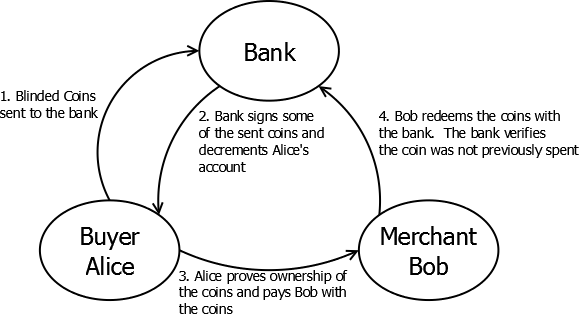
\includegraphics[scale=0.30]{images/digicash.png}
\caption{Digicash protocol.}
\label{fig:tor-end-to-end}
\end{center}
\end{figure}

The second method outlined is ``untraceable checks''.  The idea builds upon the “untraceable coins” idea by giving Alice has a roll of coins.  Alice can spend them by indexing the roll of coins by the purchase amount and revealing that to the merchant.  Alice is then refunded the rest of the amount by the bank by creating a separate transaction to pay herself.

Compact E-Cash builds upon the framework that Chaum creates with Untraceable Electronic Cash by creating a coin that can be used repeatedly a limited number of times. The system is comprised of a “withdrawal protocol”, a “spending protocol”, and a “double spending” check.  The withdrawal protocol involves the user creating a private key as well as the coin’s serial number and blinding value. The bank then signs the values and decrements the user’s account accordingly. The spending protocol has the user give the merchant the coin’s serial number, the merchant’s random number challenge, and a double-spending value based on the user’s private key, the random number challenge, and the blinding value.  The user also gives the merchant two non-interactive proofs.  The first proof is that the committed coin was signed by the bank.  The second proof verifies that the coin’s serial number and double spending number correspond to the commitment as well. The merchant then reveals this information to the bank for payment. In order to protect the user’s privacy, the serial number that is revealed to the merchant is encrypted using the user’s private key. In order to prevent the user from cheating, if the same coin is used over the limited number of uses, the bank is able to infer the secret key of the user, decrypt the serial number of the coin, and identify the user. This also means that the user can re-use coins a number of times without the bank being able to identify the user.
 
The Compact E-Cash system allows for users to create coins that can be used multiple times. The coins do not reveal the spending habits of the user if the user does not try to cheat and re-use the same coin too many times. The drawbacks are that there must be a central bank to issue coins and verify transactions. Also, each time a coin is used is a separate transaction even if the user spends multiple coins with the same merchant.

In both systems, privacy is maintained by blinded coins. If the user uses the system honestly and does not double spend, then the bank cannot reveal the identity of the user based on the coins used. Furthermore, because the coins are indistinguishable, the bank is unable to create profiles based on the location the coins were spent.

A mature form of the “untraceable coins” is the Mondex Smart Card. The bank issues secure cards embedded with an integrated circuit. The cards store “value” on the card. The “value” is incremented when money is transferred onto the card and decremented when the card is used for payment or deposit. In essence, if Alice pays Bob 5 coins, Alice’s card will destroy 5 coins and Bob’s card will create 5 coins. This makes the individual coins impossible to track. However, both Alice and Bob’s cards will have a transaction ledger that ties Alice’s and Bob’s cards to the transaction. Similar to a Bitcoin address, the card provides limited privacy as it separates the user from the coins being spent. However, merchants are able to create purchasing profiles based on transaction logs and the card’s internal identification. Furthermore, the system does not prevent merchants from sharing purchasing information with the issuing bank to match card identification numbers with an identity. In this way, the Mondex Smart Card system is less anonymous than other cryptocurrencies and does not provide any guarantees of privacy.

HashCash was originally designed to stop the waste or abuse of internet resources. HashCash requires the actor, Alice, to provide a proof-of-work before allowing an action such as sending an email. The idea is to add a cost to the action to prevent abuse. HashCash now has been incorporated into Bitcoin and similar cryptocurrency systems in the mining process as the proof-of-work protocol, but is not used as a currency system by itself. There are three protocols and two public variables in the original interactive HashCash system. The public variables are a hash function, $H(\cdot)$, and the length parameter $w$. In the Challenge protocol, the server, Bob, sends Alice the service name $s$ and a random challenge value $c$. Alice runs the Mint protocol to run a brute-force search for the value $x$. The hash of $s|c|x$, where $|$ represents concatenation, creates a value with $w$ leading zeroes. After Alice sends $x$ to Bob, Bob runs the Verify protocol to verify Alice’s work. If Verify succeeds, Alice is allowed to perform her action using the requested service. HashCash improvements include replacing the service name and challenge with a fixed output string and requiring Alice to find a collision. The proof-of-work can be considered a currency as it is used to create a transaction. If used in this way, HashCash does provide slightly better privacy than Bitcoins. Proofs-of-work are public knowledge, but HashCash does not have a ledger and therefore new nodes do not have access to the history of work.

\begin{figure}
\begin{center}
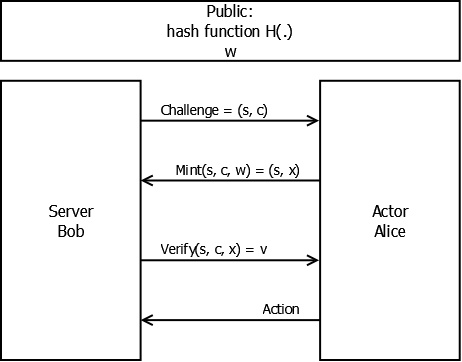
\includegraphics[scale=0.40]{images/hashcash.png}
\caption{Hashcash protocol.}
\label{fig:tor-end-to-end}
\end{center}
\end{figure}

Other alternative cryptocurrencies are based off the Bitcoin system, but only Zerocoin increases privacy. The other systems do not improve or reduce the privacy as compared to Bitcoin. Litecoin is the most similar to Bitcoin as it only differs in a few aspects. The first difference is that Litecoin uses scrypt instead of SHA-256, which is used in Bitcoin. Second, Litecoin has faster block times which decreases the time needed for a transaction confirmation. Finally, Litecoin increases the total number of coins available to be mined. Peercoin combines the HashCash proof-of-work method of mining coins with a second method, proof-of-stake. Proof-of-stake uses the notion of coin age. The coin age of a wallet is the sum of the lengths of time since a coin’s previous transaction. If Alice received 4 coins 2 days ago, then her wallet’s coin age would be 8 coin-days. In proof-of-stake, one hash per unspent wallet-output is created each second. Whereas the proof-of-work protocol uses a fixed hash target, proof-of-stake uses a variable hash target that scales inversely with coin age. If Alice finds an accepted value, she creates a transaction paying herself and is awarded one percent of her transaction as a reward. Being that her coins were used in a transaction, the mining process resets the coin age of Alice’s wallet. Namecoin is a cryptocurrency based off Bitcoin in the sense that the coins are used to register and transfer domain names. Namecoin is designed as a decentralized DNS. The ledger, which already contains coin transactions, will also contain DNS transactions such as the creation or purchase of a domain name and the associated IP address.

Unlike the previous cryptocurrencies which are based on the transference of “value”, Ripple is based on the transference of “debt”. Ripple is comprised of two parts. The first part involves a web-of-trust between nodes. Alice determines how much she trusts Bob and Charlie and then extends the maximum debt she is willing to accept from them. Suppose Charlie owes Alice 5 coins and Alice wanted to pay Bob 5 coins, but Bob only trusts Alice with a debt of 2 coins. If Bob trusts Charlie with a debt of 3 coins, Alice can send an IOU for 2 coins from her and an IOU for 3 coins from Charlie. Bob receives an IOU totaling 5 coins from which he can collect from Alice and Charlie at a later date or use to make payments to someone else.

\begin{figure*}[ht]
\begin{center}
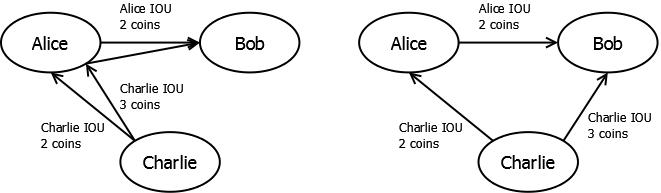
\includegraphics[scale=0.40]{images/ripple.png}
\caption{Ripple debt network.}
\label{fig:tor-end-to-end}
\end{center}
\end{figure*}

The second part of Ripple is to facilitate transactions where no web-of-trust exists. This is done through “gateway” nodes. Gateways act as publically known trusted nodes analogous to banks. If Alice wanted to pay Bob 5 coins, but Bob only trusts a gateway, then Alice can send 5 coins to the gateway and the gateway will credit Bob 5 coins. Unlike the first part of Ripple, gateways use stores of “value” instead of debt. Ripple is as private as Bitcoins as transfers of debt or credit between addresses is public knowledge, but no registry ties addresses to people. The exception is if Ripple deals with real world currency. Ripple is currency agnostic and therefore gateways are free to use real world currency as an exchange medium. In this case, gateways require personal information from the user and are able to link users to addresses and transactions.

